\documentclass[11pt,oneside]{article}
\usepackage{geometry}			% See geometry.pdf to learn the layout options.								
\geometry{letterpaper}			% ... or a4paper or a5paper or ... 
\usepackage[parfill]{parskip}	% Activate to begin paragraphs with an empty  line rather than an indent
\usepackage{mathpazo}
\usepackage{amsmath}		
\usepackage{graphicx}
\usepackage{hyperref}

\usepackage[font={bf,footnotesize},textfont=md,margin=30pt,aboveskip=0pt,belowskip=0pt]{caption}

\begin{document}


\begin{center}
	\textbf{Assignment 3: Lorenz equations - GEOG 5100}\\
	{\itshape Cameron Bracken} - September 27, 2009
\end{center}


\begin{enumerate}
\item A strange attractor is a region of the state space of a nonlinear differential equation to which all solutions are attracted.  Strange attractor cannot exist in less than 3 dimensions.  

\item 
\begin{enumerate}
	\item[a)] The two solutions behave similarly in that they both spiral around the attractor moving from one basin to another.  They also do not behave in exactly the same way either.  
	\item[b)] The number of times the solution stays in either basin is erratic and not predictable by inspection. This has to do with the inherent unpredictability of chaotic systems.
	\item[c)] A weather system, if indeed chaotic, may never be able to be predicted accurately after some time horizon, no matter how good the models or data. 
	\item[d)] Climate prediction may deal more with averages conglomerate numbers which might be less influenced by the erratic behavior of individual weather systems. 
\end{enumerate}

\item Phase space is the space made up of the dependent variables in a dynamical system.  That is in the dynamical system $\mathbf{\dot{x}} = \mathbf{f}(\mathbf{x})$, $\mathbf{x}$ defines the phase space. Solution trajectories travel through phase space with the passing of time. 

\item 
\begin{enumerate}
	\item[a)] An initial condition is a point in phase space which defines the starting conditions of a dynamical system. 
	\item[b)] On the first time step where the equations reference a time in the past, the initial conditions are used.  That is when $t=0$, then $\mathbf{x}_{t-1}$ refers to the initial conditions. 
	\item[c)] Every dependent variable needs an initial condition. 
	\item[d)] Tunable parameters in the Lorenz model are $\sigma, r$ and $b$.  Though in practice, since $\sigma$ and $r$ represent physical parameters, $b$ might be the only true tunable. 
\end{enumerate}

\item The non-linear terms in the Lorenz equations:
\begin{align}
\dot{x}&=\sigma(y-x)\\
\dot{y}&=rx-y-xz\\
\dot{z}&=xy-bz
\end{align}
are the $xz$ and $xy$ terms in equations 2 and 3. 

\item Determinism in a physical system refers a system following a set of physical laws which can typically be described with closed form equations. More precisely it refers to a lack of randomness.

\item `Orderly disorder' refers to the behavior of a chaotic system with an attractor.  The behavior of the system is orderly in that a box can be put around the attractor and all solutions will eventually end up in that box.  The disorder refers to the movement of solutions within that box or around the attractor, which is unpredictable in the long term. 

\item  The change in the initial conditions was in the forth decimal place of his initial conditions, due to truncation error. 

\item Self similarity is a property of an attractor which has fine geometrical structure on an arbitrarily small scale.  In this way attractor are intimately related to fractals. 

\item A classic example of a fractal is the cantor set:

\begin{figure}[!htbp]
   \centering
	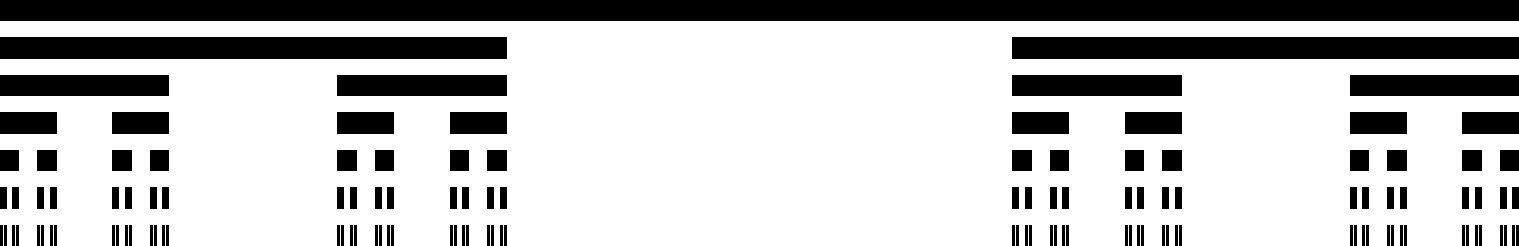
\includegraphics[width=.85\textwidth]{Cantor_set_in_seven_iterations.pdf}
   \caption{Seven iteration of the Cantor Set (Source: \url{http://en.wikipedia.org/wiki/Cantor_set})}
\end{figure}

This set is created by starting with a continuous number line $[0,1]$ and subtracting the middle third $(1/3,2/3)$.  Then the middle third of the remaining pieces is removed and the process repeats recursively. The remaining set has some very interesting properties. For example, the removed pieces can be shown to add up to 1!

\item 
\begin{enumerate}
	\item[a)] The Euler and Runge-Kutta methods refer to numerical solution techniques for ordinary differential equations. They are used to obtain solutions to equations that may not have an analytical solution. 
	\item[b)] The Runge-Kutta method is more accurate than the Euler method but also more computationally more efficient.  The Euler method used fewer functional evaluations to calculate derivates. 
	\item[c)] Figure 16.1.2 describes the midpoint method for numerically solving ODEs. In this method, derivates at two points in between the actual three evaluation points are used to get more accurate estimates of derivates. 
	\item[d)] A second order method uses two functional evaluations at each time step while a fourth order method uses four. In general a fourth order method is more accurate, but more computationally intense. 
\end{enumerate}

\item
\begin{enumerate}
	\item[a)] Forward difference form:
\begin{align}
	x_{i+1}&={\Delta t}(\sigma(y-x))+x_i\\
	y_{i+1}&={\Delta t}(rx-y-xz)+y_i\\
	z_{i+1}&={\Delta t}(xy-bz)+z_i
\end{align}
	\item[b)] Backward difference form:
\begin{align}
	x_{i}&={\Delta t}(\sigma(y-x))+x_{i-1}\\
	y_{i}&={\Delta t}(rx-y-xz)+y_{i-1}\\
	z_{i}&={\Delta t}(xy-bz)+z_{i-1}
\end{align}
\end{enumerate}



\end{enumerate}


\end{document}
